\section{Implementation}
This section will deal with the more technical aspects of this case study. From now on we will list topics that have to do with the implementation of the simple Http server.

\subsection{Defining the required GNAT Project File Specification}
The specifications list the following requirements for the directory structures: 
\begin{table}
\begin{center}
\begin{tabular}{|c|l|}
\hline
src & The directory to contain the sources \\ \hline
obj & The directory to contain the compiler output \\ \hline
bin & The directory to contain the binaries \\ \hline
obj/debug & \parbox{10cm}{The non-optimized compiled binaries with debug info are stored here. You can notice this in the GPR file, where the `-g' flag is given to the compiler.} \\ \hline
obj/release &  \parbox{10cm}{The optimized compiled binaries without debug information. You  can notice this in the GPR file, where the `O2' flag is given to the compiler.} \\ \hline
tests & The directory to contain the tests \\ \hline
\end{tabular}\end{center}
\caption{Directory Structure Specification for GPR File}
\end{table}
\subsubsection{GNAT Project File}
Here is the project file we will be using.
\lstinputlisting[caption=GNAT Project File,language=Ada]{../axios/axios.gpr}
Notice that some of the flags for the compiler in both release, and debug modes are the same flags used for GNU C++ compiler. We explain each section with a little more detail.

\paragraph{Directory Structure}The directory structure is as outlined on the previously demonstrated table. We see these defined in the GPR file by the names of \textbf{Source\_Dirs}, \textbf{Exec\_Dir}. Because of the definition of the Object file directories for a debug and release version, we also get the ``obj/release'' and ``obj/debug'' directories, as previously required. A Simple hello world application would yield the following structure, for example: 

\lstinputlisting[caption=Directory Structure,language=ruby]{src/misc/dir-struct.txt}

\paragraph{Flags} There are many flags that can be set for the compilation and linking process. The manual covers a lot of them, but the ones used are explained.

\subparagraph{Builder} Notice the "package Builder is ..." line. We define the flags that should be used by the builder (gnatmake), when invoked.

\subparagraph{Executable} This is to specify the output name of the binary once the whole project is compiled.

\subparagraph{Compiler} Notice the "package Compiler is ..." line. This contains the flags for the actual compiler. We have two flags `-g', and `-O2' that the seasoned GNU C++ compiler user would recognize instantly. The `-g' flag would be used to produce non-optimized binaries in order to contain extra information when debugging. 
The `-O2' is for optimization, and that is the reason why it is in the release case. We define a Mode\_Type which can either be one of the two literals `debug', and `release' in order to achieve this. 

\subsection{Components}
We now describe the components of the project. Figure \ref{fig:system-architecture}

\begin{figure}[hb]
\centering
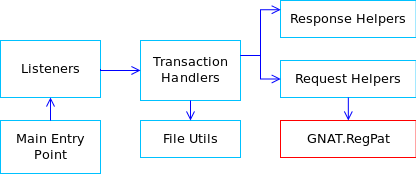
\includegraphics[width=4in]{gfx/system-architecture.png}
\caption{Overall organization of software components of Axios}
\label{fig:system-architecture}
\end{figure}


\subsubsection{Listener}
\paragraph{Specification} Here is the code listing for the listener specification
\lstinputlisting[language=Ada,caption={Simple Listener Specification}]{../axios/src/listeners.adb}

\paragraph{Implementation} Here is the code listing for the listener implementation
\lstinputlisting[language=Ada,caption={Simple Listener Body}]{../axios/src/listeners.adb}

\section{Testing}
Testing is achieved by using \textbf{AUnit} in order to do unit testing. 


